% <- percent signs are used to comment
\documentclass[12pt]{article}

%amsmath is a packaged use for typesetting math
%amsfonts is required for special fonts, e.g. blackboard bold (for denoting real numbers, etc.)
\usepackage{amsmath,amsfonts}

\usepackage{fullpage,url,amssymb,epsfig,color,xspace}

%Note: Many of the packages above have other uses beyond those used in this document

%this marks the beginning of the document. Everything before this is called the Preamble.
\begin{document}
%marks the end of the title section
\begin{center}
{\Large\bf University of Waterloo}\\
\vspace{3mm}
{\Large\bf MATH 213, Spring 2015}\\
\vspace{2mm}
{\Large\bf Assignment 6}\\
\end{center}

\section*{Question 1}
a) Draw a labelled sketch of the following function. $$f(t) = \sin t - \sin (t-2) H(t-2) + t^2H(t-3)$$

\begin{center}
  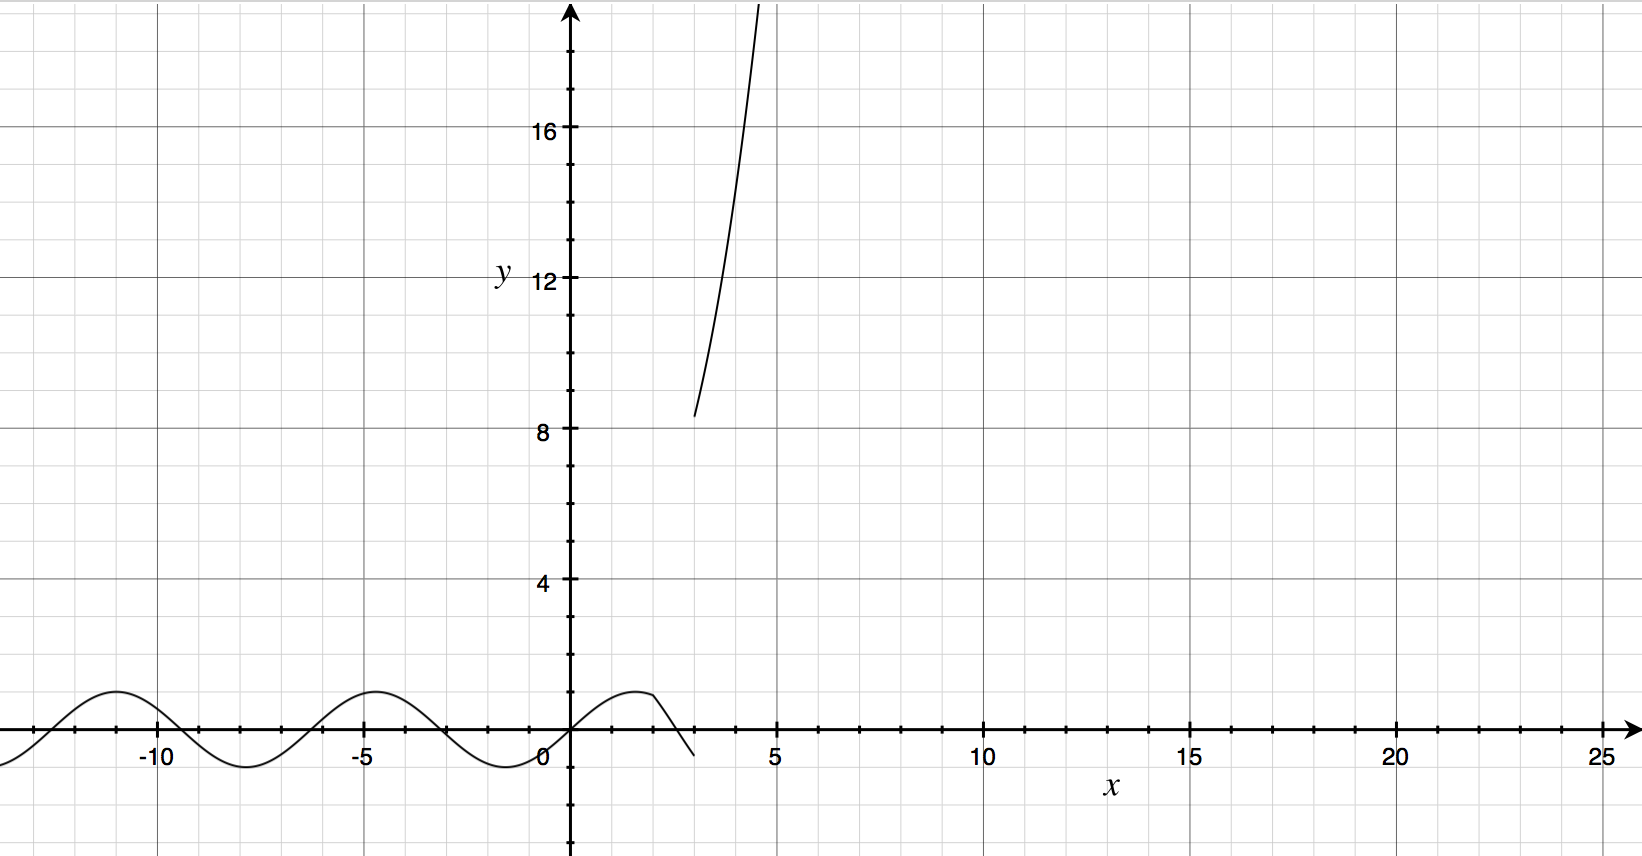
\includegraphics[scale=0.4]{q1agraph.png}
\end{center}
\hfill (2 marks)

\noindent b) Derive a single expression for $f(t)$ from the following graph. Evaluate the transform.
\begin{center}
  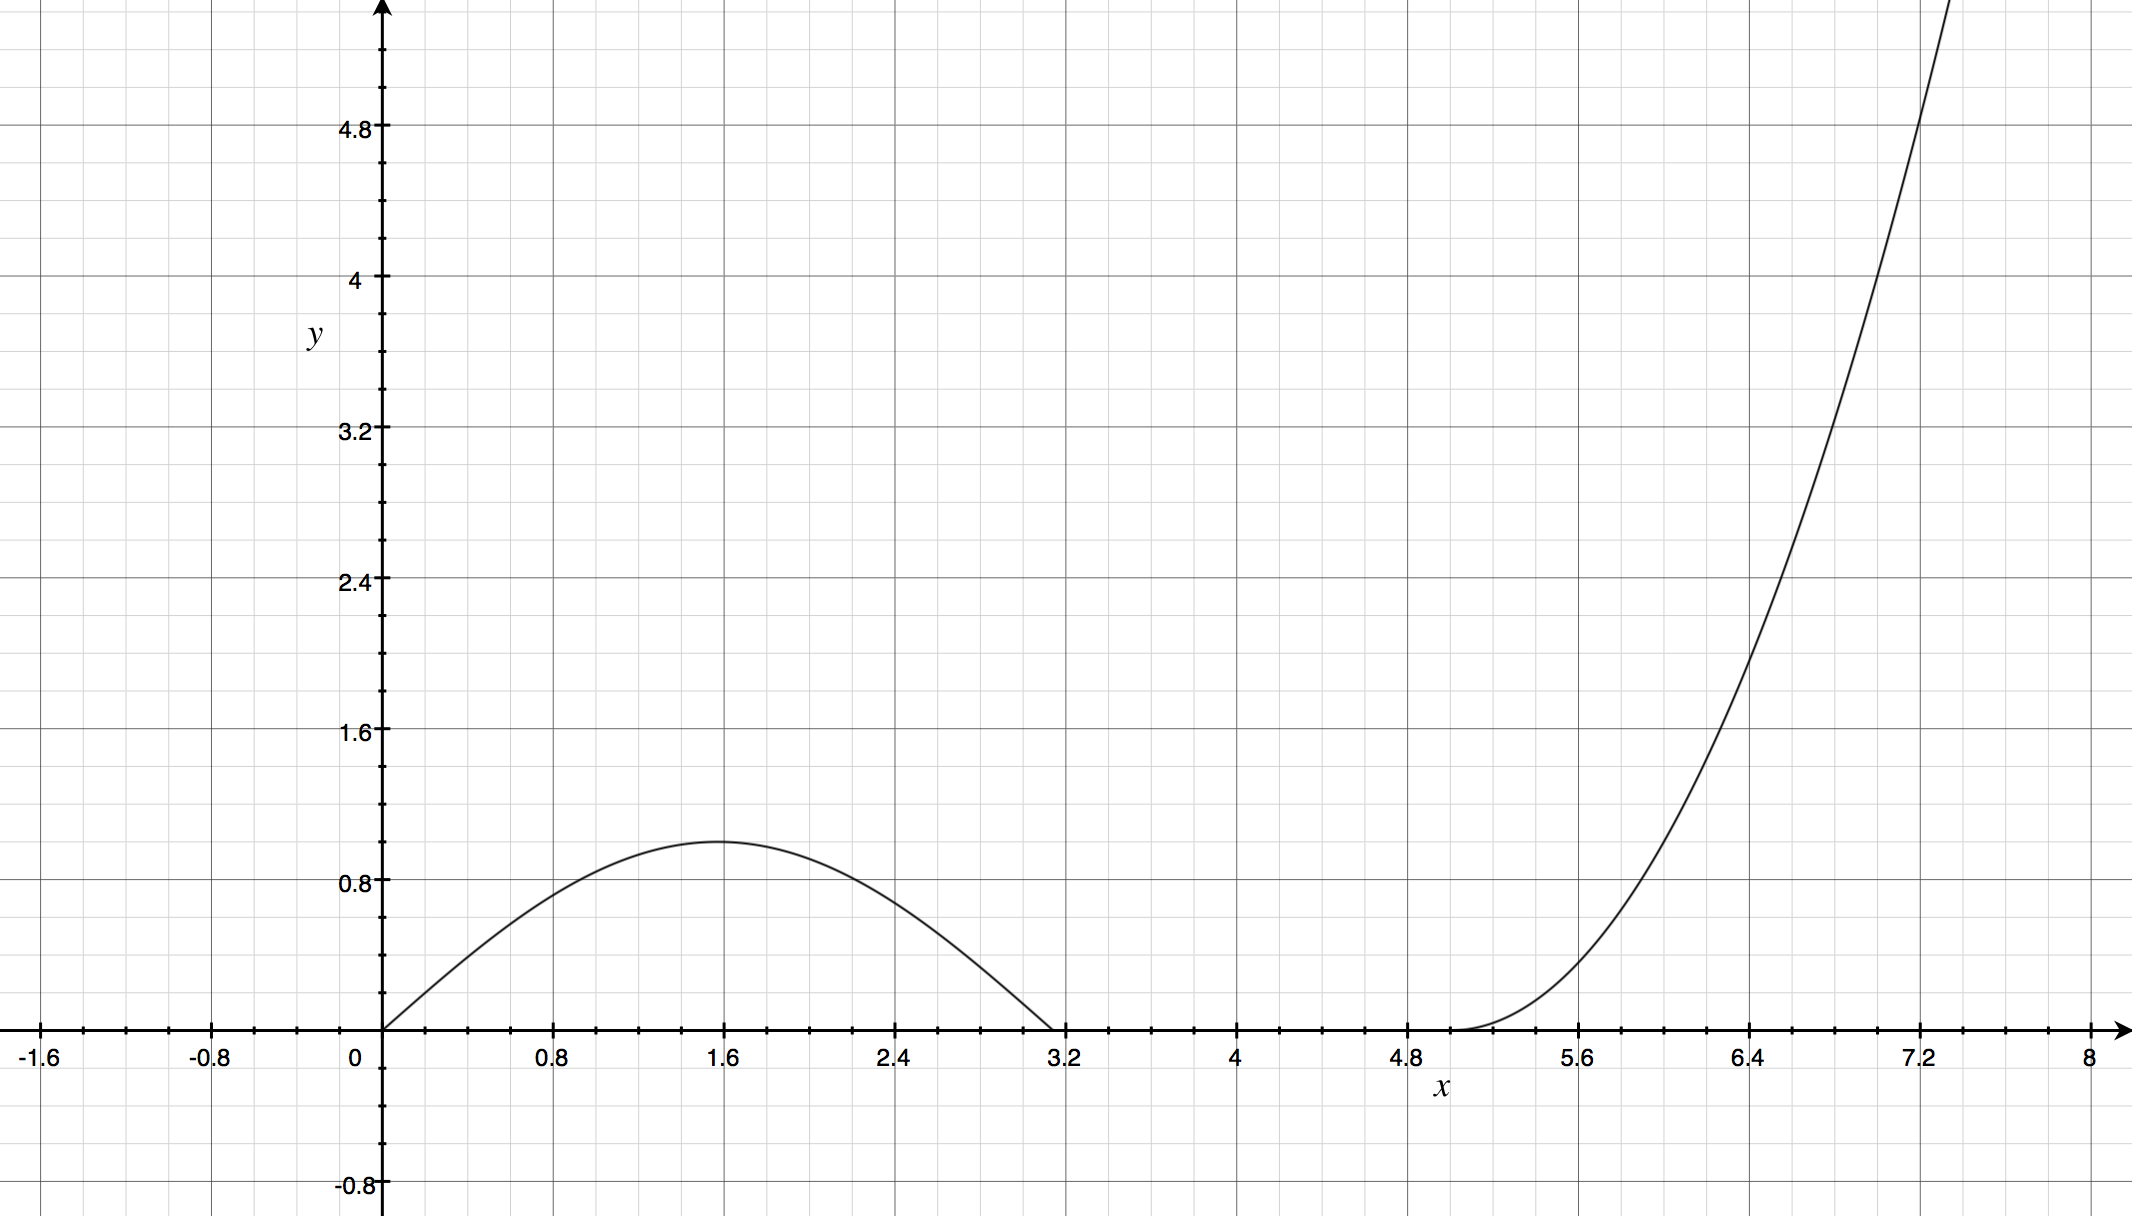
\includegraphics[scale=0.2]{q1graph.png}
\end{center}

\noindent From the graph, we get the following function, $$f(t) = \sin(x) - \sin(x-\pi)u(t-\pi) + (x-5)^2u(t-5)$$ \hfill (1 mark) \\ Taking the transform, we get $$F(s) = \frac{1}{s^2+1} - \frac{e^{-\pi s}}{s^2+1} + \frac{2e^{-5s}}{s^3}$$ \hfill (2 marks)

\section*{Question 2}

Use the Laplace transform to find the particular solution of the following functions
$$y' + y = \sin(t - 3)u(t - 3) + tu(t - 3) - 3u(t - 3), y(0) = 0$$


\noindent Where
\[
 u(t) =
  \begin{cases}
    0 &\text{when } t < 0 \\
    1 &\text{when } t \ge 0
  \end{cases}
\]

Take the Laplace of both sides:
\begin{align*}
  &y' + y = \sin(t - 3)u(t - 3) + tu(t - 3) - 3u(t - 3)
  \\ &y' + y = \sin(t - 3)u(t - 3) + (t - 3)u(t - 3)
  \\ &sY(s) + Y(s) = \frac{e^{-3s}}{s^2 + 1} + \frac{e^{-3s}}{s^2}
  \\ &(s + 1)Y(s) = e^{-3s}\bigg(\frac{1}{s^2 + 1} + \frac{1}{s^2}\bigg)
  \\ &Y(s) = e^{-3s}\bigg(\frac{1}{(s^2 + 1)(s + 1)} + \frac{1}{s^2(s + 1)}\bigg) \tag{1 mark}
\end{align*}

Use partial fraction decomposition:
\begin{align*}
  &\frac{1}{(s^2 + 1)(s + 1)} = \frac{As}{s^2 + 1} + \frac{B}{s^2 + 1} + \frac{C}{s + 1}
  \\&1 = As^2 + As + Bs + B + Cs^2 + C
  \\& A + C = 0, A + B = 0, B + C = 1
    \\& \therefore A = -0.5, C = 0.5, B = 0.5 \tag{1 mark}
\end{align*}

\begin{align*}
  &\frac{1}{s^2(s + 1)} = \frac{A}{s} + \frac{B}{s^2} + \frac{C}{s + 1}
  \\&1 = As^2 + As + Bs + B + Cs^2
  \\& A + C = 0, A + B = 0, B = 1
    \\& \therefore A = -1, B = 1, C = 1 \tag{1 mark}
\end{align*}

Take the inverse Laplace:
\begin{align*}
  &Y(s) = e^{-3s}\bigg(\frac{1}{(s^2 + 1)(s + 1)} + \frac{1}{s^2(s + 1)}\bigg)
  \\ &Y(s) = e^{-3s}\bigg(-\frac{1}{2}\frac{s}{s^2 + 1} + \frac{1}{2}\frac{1}{s^2 + 1} + \frac{1}{2}\frac{1}{s + 1} -\frac{1}{s} + \frac{1}{s^2} + \frac{1}{s + 1}\bigg)
    \\ &y(t) = \bigg(-\frac{1}{2}cos(t - 3) + \frac{1}{2}sin(t - 3) + \frac{3e^{-(t-3)}}{2} - 1 + (t - 3)\bigg)u(t - 3) \tag{2 marks}
\end{align*}

\end{document}
